\documentclass[12pt]{article}
\usepackage{graphicx}
\usepackage{amsmath}
\usepackage[a4paper, total={6in, 8in}]{geometry}
\setlength{\parindent}{0pt}
\usepackage{color}
\newcommand{\hilight}[1]{\colorbox{yellow}{#1}}


\begin{document}
	
	
	\title{Finite Element Method for The Heat equation}
	\author{Andres Chaves(), Diego Montufar()}
	
	\maketitle
	
	\begin{abstract}
		The abstract text goes here.
	\end{abstract}
	
	\section{Introduction}
	
	The finite-element method provides an alternative that is better suited for complex systems.
In contrast to finite-difference techniques, the finite-element method divides the solution domain into simply shaped regions, or "elements". An approximate solution for the PDE can be developed for each of these elements. The total solution is then generated by linking together, or "assembling", the individual solutions taking care to ensure continuity at the interelement boundaries. Thus, the PDE is satisfied in a piecewise fashion.

Although the particulars will vary, the implementation of the finite-element approach usually follows a standard step-by-step procedure.

1. Discretization
2. Element Equations
3. Assembly
	
	
	\section{Problem Statement}
	
The heat equation can be used to describe the temperature variation through a
solid body. The equation derives from the principle of conservation of energy and
and gives rise to a second order linear PDE of the form:
	
	\begin{equation}\label{eq:equation}
		\rho C \frac{\partial T}{\partial t} = k \nabla^2 T
	\end{equation}
	
Where $T$ is the temperature $[K]$,$\rho$ is the mass density $[kgm^3]$, $C$ is the specific heat capacity $[Jkg^{-1}K^{-1}]$, and $k$ is the thermal conductivity $[Wm^{-1}K^{-1}]$. For this particular implementation the computational domain will describe cooling fins on top of a central processing unit
and will be defined by an unstructured tetrahedral grid. We assumed that the cooling fins are made from pure copper, having the properties $\rho = 8954kgm^3$, $C = 380Jkg^{-1}K^{-1}$, and $k = 386Wm^{-1}K^{-1}$. 

In this particular case the CPU creates a constant heat flux $Q_{cpu}$ , given by:

	\begin{equation}
		Q_{cpu} = k \nabla T
	\end{equation}
	
which defines a Neumann boundary condition on the base of the domain and $Q_{cpu} = 40,000Wm^{-2}$. For the remaining boundary of the cooling fins we assumed a convection boundary condition, given by:

	\begin{equation}
		Q_{air} = k \nabla T = h(T-T_{air})
	\end{equation}

which defines a Robin boundary condition. Here we assumed that the convection coefficient $h = 100W/m^2K^{-1}$ and the ambient temperature $T_{air} = 300K$. Defining the initial temperature of the cooling fins as ambient, the main goal is  to simulate the temperature rise in the domain $t \in [0,100]s$ and determine the maximum steady state temperature of the cooling fins.
	

%----------------------------------------------------------	
	
	\section{Governing Equations}

In order to solve the Heat Equation using the Finite Element method, we are going to start by deriving the weak form of Equation (1). Applying this numerical method implies a series of steps until we get a global system of equations that must be assembled in order to compute the solution. So we are going to follow the next steps:

\begin{enumerate}
  \item Derive the weak form of the Heat Equation by applying the Galerking Weighted residual method.
  \item Express our field variable $T$ and its derivatives in terms of the shape functions for a linear tetrahedral element.
  \item Assemble the global system of equations.
\end{enumerate}

\subsection{Galerking Weighted residual method}
Weighted residual methods assume that a solution can be approximated analytically or piecewise analytically. The idea of this method is that we can multiply the residual by a weighting function and force the integral of the weighted expression over the domain to vanish:

	\begin{equation}
		\int\limits_{\Omega} W(x) r(x) d\Omega = 0
	\end{equation}
	
	We understand the residual as a continuous function of space.  In the Galerking method the weight functions are chosen to be identical to the trial functions where the trial function is our assumed approximate solution for the PDE which takes the form:
	
	

	\begin{equation}
		\phi(x) = \sum_{n=0}^N a_n(x)p_n(x), \quad \text{Where}  \quad W_n(x)=p_n(x)
	\end{equation}		
	
	Applying equation (4) to the Heat Equation (1) we have:

$$
r={\rho C \frac{\partial T}{\partial t} - k \nabla^2 T}
$$

	$$\int\limits_{\Omega} W ({\rho C \frac{\partial T}{\partial t} - k \nabla^2 T}) d\Omega = 0$$
	
	This is an appropriate time to include the convection term into our equation and expanding terms we get:
	
	\begin{equation}
		\int\limits_{\Omega} W \rho C \frac{\partial T}{\partial t} d\Omega - \int\limits_{\Omega} W k \nabla^2 T d\Omega + \int\limits_{\Omega} W Q_{air} d\Omega = 0
	\end{equation}

	We can modify the diffusive second order term by applying the product rule for derivatives which is defined by:
	
\begin{align*}
\nabla\cdot(W\nabla T) &= \nabla W \cdot\nabla T+W \nabla \cdot\nabla T \\
&=\nabla W \cdot\nabla T+W \nabla^2 T
\end{align*}

In our second term of Equation (6): Applying the product rule, rearranging, and integrating over the domain we get:
		
	\begin{equation}
	\int\limits_{\Omega} W k \nabla^2 T d\Omega = \int\limits_{\Omega} \nabla \cdot ({Wk\nabla T}) d\Omega - \int\limits_{\Omega} \nabla W \cdot k \nabla T d\Omega
	\end{equation}

	in order to eliminate second order terms of the Equation (7), another important concept we are going to use is the theorem of divergence which can be expressed as follows:
	
	$$
	\int\limits_{\Omega} \nabla^22 T d\Omega = \int\limits_{\Gamma} \nabla T \cdot d\Gamma 
	$$
	
Now, we can make use of the Divergence Theorem and apply it to the second order term of Equation (7) as follows:	
	
	\begin{equation}
	\int\limits_{\Omega} k W \nabla^2 T d\Omega = \int\limits_{\Gamma} {kW\nabla T} \cdot d \mathbf{\Gamma} - \int\limits_{\Omega} k \nabla W \cdot \nabla T d\Omega
	\end{equation}

	Substitute Equation (8) in (6) we get:
	
	\begin{equation}
	\int\limits_{\Omega} \rho C W \frac{\partial T}{\partial t} d\Omega -  \int\limits_{\Gamma_{Base}} {kW\nabla T} \cdot d \mathbf{\Gamma} - \int\limits_{\Omega} k \nabla  W \cdot \nabla T d\Omega + \int\limits_{\Gamma_{Fins}} W Q_{air} d\Gamma = 0
	\end{equation}
	
	The important point here is that applying the Galerkin method of weighted residuals this way means that for every element we get a 'sub' system of equations local to each element and in terms of the local nodal values $1...N_n$, that must be assembled
into a global system of equations with global indices $1...N_p$
		
	Then we can see the second term in the equation corresponds to the value of $Q_{cpu}$ as stated in the model problem. In contrast to other methods, the Neumann boundary conditions are automatically incorporated into the integral form of the PDE. Rearranging terms we get the Weak form of the Heat Equation:

	\begin{equation}
	\int\limits_{\Omega} \rho C W \frac{\partial T}{\partial t} d\Omega + \int\limits_{\Omega} k \nabla W \cdot \nabla T d\Omega = \int\limits_{\Gamma_{Base}} {kW\nabla T} \cdot d \mathbf{\Gamma} - \int\limits_{\Gamma_{Fins}} W {h(T-T_{air})} d\Gamma
	\end{equation}

The overall global system of equations to solve our generic scalar transport equation is then given by:

	\begin{equation}
	\sum_{n=1}^{N_p}\int\limits_{\Omega} (W \rho C \frac{\partial T}{\partial t} + \nabla W \cdot k \nabla T) d\Omega = \sum_{n=1}^{N_p} \int\limits_{\Gamma_{Base}} {Wk\nabla T} \cdot d \mathbf{\Gamma} - \sum_{n=1}^{N_p} \int\limits_{\Gamma_{Fins}} W {h(T-T_{air})} d\Gamma
	\end{equation}


	\subsection{Shape functions}

One of the fundamental steps in a finite element analysis is the discretization of a continuous body containing infinite number of points in the surface into a discrete model with a limited number of points (or nodes) in the surface. The shape of the body between these nodes its approximated by functions. These functions are known as shape functions, and allow us to relate the coordinates of every point of a finite element with the positions of its nodes.

Thinking of $T$ most generally as being a continuous function of space and time, we will write the assumed solution in the form:

\begin{equation}
T(\mathbf{x},t) = \sum_{n=1}^{N_n} \eta_n(\mathbf{x})T_n(t)
\end{equation}

Where $\eta_n$ are known as the \textsl{shape functions}, which are functions of spatial location only, while the nodal values of $T$ are functions of time only. 

If we now substitute in our assumed form of the solution from Equation (10), and consider the domain of integration to be the domain of an element itself, the weighted residual expression can be rewritten using Einstein summation notation as:

	\begin{equation}
	\int\limits_{\Omega_e} \eta_p\eta_q \rho C \frac{\partial T}{\partial t} d\Omega + \int\limits_{\Omega_e} k \nabla \eta_p \cdot \nabla \eta_q T_q d\Omega = \int\limits_{\Gamma_{e}}{k\eta_p\nabla T} \cdot d \mathbf{\Gamma} - \int\limits_{\Gamma_{e}}h\eta_p(\eta_qT_q-T_{e}) d\Gamma
	\end{equation}

Then the overall System of Equations to solve the Heat Equation is the given by:

\begin{equation}
	\sum_{e=1}^{N_e}  \int\limits_{\Omega_e} \bigg(\eta_p\eta_q \rho C \frac{\partial T_q}{\partial t} d\Omega + k \nabla \eta_p \cdot \nabla \eta_q T_q\bigg) d\Omega = \sum_{e=1}^{N_e} \int\limits_{\Gamma_{e}}{k\eta_p\nabla T} \cdot d \mathbf{\Gamma} - \sum_{e=1}^{N_e} \int\limits_{\Gamma_{e}}\eta_p h (\eta_qT_q-T_{air}) d\Gamma
	\end{equation}

We can then rewrite the system of equations in the form:

\begin{equation}
 M\dot{T} = KT + s
\end{equation}

Where $M$ represents the Mass matrix, $K$ the Stiffness Matrix, both have size of $N_p$x$N_p$ and finally the $s$ term that is the load vector with size $N_p$x$1$. For the Heat Equation we can recognize each term of Equation(15) in the Equation (13) as follows:

\begin{equation}
 M_{pq}^e = \int\limits_{\Omega_e} \eta_p\eta_q \rho C d\Omega
\end{equation}

\begin{equation}
 K_{pq}^e = -\int\limits_{\Omega_e} k \nabla \eta_p \cdot \nabla \eta_q d\Omega - h \int\limits_{\Gamma_e} \eta_p \eta_q d\Gamma
\end{equation}

\begin{equation}
 S_{p}^e = h T_{air} \int\limits_{\Gamma_e} \eta_p d\Gamma + k \int\limits_{\Gamma_{e}}{\eta_p\nabla T} \cdot d \mathbf{\Gamma}
\end{equation}

For this case we are going to use tetrahedral elements, which means we are going to have 4 nodes in a 3D \hilight{element as shown in Figure()}. In order to derive the corresponding shape functions we begin by assuming a trial solution which takes the form:

\begin{equation}
T(x,y,z) = a_0+a_1x+a_2y+a_3z
\end{equation}

Where $a_0$,$a_1$,$a_2$ and $a_3$ are scalar coefficients. This is essentially the 3D equivalent of the trial solution to a triangular element. If we apply this trial solution in every node of the element we'll get:

\begin{equation}
\begin{Bmatrix} T_1 \\ T_2 \\ T_3 \\ T_4 \end{Bmatrix} = 
\begin{bmatrix} 1 & x_1 & y_1 & z_1 \\ 1 & x_2 & y_2 & z_2 \\ 1 & x_3 & y_3 & z_3 \\ 1 & x_4 & y_4 & z_4\end{bmatrix}
\begin{Bmatrix} a_0 \\ a_1 \\ a_2 \\ a_3 \end{Bmatrix} =
\begin{bmatrix} \mathbf{p_1} \\ \mathbf{p_2} \\ \mathbf{p_3} \\ \mathbf{p_4} \end{bmatrix}\mathbf{a} = C\mathbf{a}
\end{equation}

Where $p_n=\{1 \thinspace x_n \thinspace y_n \thinspace z_n\}$, $C$ will be a square $4$x$4$ matrix and we can solve for the unknown parameters by computing $\mathbf{a}=C^{-1}\mathbf{T}$. Doing so we can find our shape functions by substituting these coefficients back into our trial solution, So we can factor out the nodal values and rewrite the solution in the form:

\begin{equation}
T(x,y,z) = \sum_{n=1}^{N_n} \eta_n{(x,y,z)} T_n = \eta_1 T_1 + \eta_2 T_2 + \eta_3 T_3 + \eta_4 T_4
\end{equation}

Where the shape functions for the linear tetrahedron are:

\begin{center}
  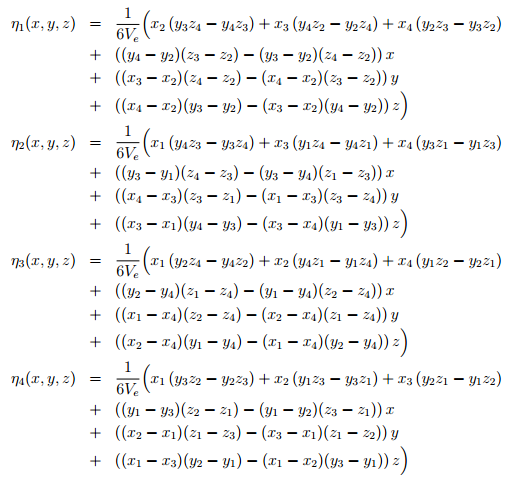
\includegraphics[width=0.8\textwidth]{ShapeFunctions}
\end{center}

Where $V_e$ is the volume of the element and is defined in terms of its nodal coordinates as:

\begin{equation}
6V_e=\begin{bmatrix} 1 & x_1 & y_1 & z_1  \\ 1 & x_2 & y_2 & z_2  \\ 1 & x_3 & y_3 & z_3 \\ 1 & x_4 & y_4 & z_4 \end{bmatrix}
\end{equation}

And we could express the derivatives of the shape functions as:

\begin{center}
  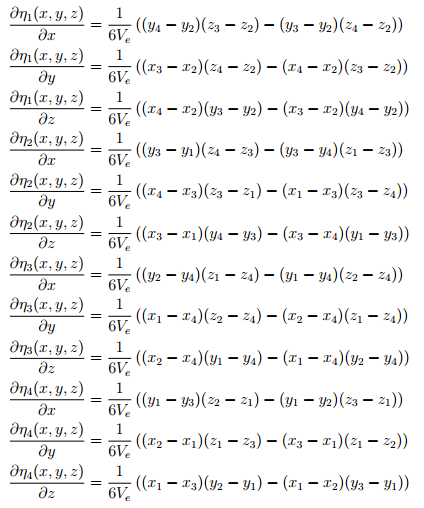
\includegraphics[width=0.7\textwidth]{GradientShapeFunctions}
\end{center}

Furthermore, we have the integration formulae defined for the linear tetrahedron:

\begin{equation}
 \int\limits_{\Omega_e} \eta_p^a \eta_q^b \eta_r^c \eta_s^d d{\Omega}=
 \frac{a!b!c!d!6\Omega_e}{(a+b+c+d+3)!}
\end{equation}

and:

\begin{equation}
 \int\limits_{\Gamma_e} \eta_p^a \eta_q^b \eta_r^c  d{\Omega}=
 \frac{a!b!c!2\Gamma_e}{(a+b+c+2)!}
\end{equation}

Where for the 3D case $\Omega_e$ and $\Gamma_e$ represent the volume and face area of a tetrahedron respectively.

Let's first
consider the integration of the shape functions as required in the mass matrix from Equation (16):

$$
M_{p,q}^e = \rho C \int\limits_{\Omega_e} \eta_p \eta_q d\Omega
$$

Remembering that p and q are in the range of 1 to 4 for the linear tetrahedral element,
what we end up with is a local or 'sub' matrix $M_e$, which for our linear tetrahedral
element will be a 4 x 4 matrix. In order to evaluate each term in the matrix we
simply input the values of p and q to the integration formula in Equation (23). For
the case where p and q are equal (i.e. for elements on the main diagonal) we get:

\begin{align*}
 M_{p,p}^e & = \rho C  \int\limits_{\Omega_e} \eta_p \eta_p d\Omega \\
              	& = \rho C \int\limits_{\Omega_e} \eta_p^2 \eta_q^0 \eta_r^0 \eta_s^0 d{\Omega}=
 \frac{\rho C 2!0!0!0!6\Omega_e}{(2+0+0+0+3)!} \\
 				& = \frac{2\rho C \Omega_e}{20}
\end{align*}

For the case where p and q are not equal (i.e. for elements off the main diagonal) we get:

\begin{align*}
 M_{p,q}^e & = \rho C \int\limits_{\Omega_e} \eta_p \eta_q d\Omega \\
              	& = \rho C \int\limits_{\Omega_e} \eta_p^1 \eta_q^1 \eta_r^0 \eta_s^0 d{\Omega}=
 \frac{\rho C 1!1!0!0!6\Omega_e}{(1+1+0+0+3)!} \\
 				& = \frac{\rho C \Omega_e}{20}
\end{align*}

So we can write a single expression for the any element in our local mass matrix as:

$$
M_{p,q}^e = \frac{\rho C (1+\delta_{pq})}{20}
$$

which is simple enough that we could write out the whole thing as:

\begin{equation}
M^e = \frac{\rho C \Omega_e}{20}{\begin{bmatrix} 2 & 1 & 1 & 1 \\ 1 & 2 & 1 & 1 \\ 1 & 1 & 2 & 1 \\ 1 & 1 & 1 & 2 \end{bmatrix}}
\end{equation}

Considering now the contribution of the diffusive term to the stiffness matrix, and writing shape function derivative terms in the form of a column vector with modulo 3 notation for compactness we have:


\begin{align*}
 -k\int\limits_{\Omega_e} \nabla \eta_p \cdot \nabla \eta_q d\Omega &= \\ 
 &= -k\int\limits_{\Omega_e} \frac{1}{6\Omega_e} 
 \begin{Bmatrix} 
 (y_{p+3}-y_{p+1})(z_{p+2}-z_{p+1})-(y_{p+2}-y_{p+1})(z_{p+3}-z_{p+1}) \\
 (x_{p+2}-x_{p+1})(z_{p+3}-z_{p+1})-(x_{p+3}-x_{p+1})(z_{p+2}-z_{p+1}) \\
 (x_{p+3}-x_{p+1})(y_{p+2}-y_{p+1})-(x_{p+2}-x_{p+1})(y_{p+3}-y_{p+1}) \\
 \cdots
 \end{Bmatrix} \\
 &\dot{•} 
 \frac{1}{6\Omega_e} 
 \begin{Bmatrix} 
 (y_{q+3}-y_{q+1})(z_{q+2}-z_{q+1})-(y_{q+2}-y_{q+1})(z_{q+3}-z_{q+1}) \\
 (x_{q+2}-x_{q+1})(z_{q+3}-z_{q+1})-(x_{q+3}-x_{q+1})(z_{q+2}-z_{q+1}) \\
 (x_{q+3}-x_{q+1})(y_{q+2}-y_{q+1})-(x_{q+2}-x_{q+1})(y_{q+3}-y_{q+1}) \\
 \cdots
 \end{Bmatrix}
\end{align*}

Performing the Integration we get:

\begin{equation}
\begin{aligned}
-k\int\limits_{\Omega_e} \nabla \eta_p \cdot \nabla \eta_q d\Omega &= \\
 & -\frac{k}{36\Omega_e^2} 
 \begin{Bmatrix} 
 (y_{p+3}-y_{p+1})(z_{p+2}-z_{p+1})-(y_{p+2}-y_{p+1})(z_{p+3}-z_{p+1}) \\
 (x_{p+2}-x_{p+1})(z_{p+3}-z_{p+1})-(x_{p+3}-x_{p+1})(z_{p+2}-z_{p+1}) \\
 (x_{p+3}-x_{p+1})(y_{p+2}-y_{p+1})-(x_{p+2}-x_{p+1})(y_{p+3}-y_{p+1}) \\
 \cdots
 \end{Bmatrix} \\
 &\dot{•} 
 \begin{Bmatrix} 
 (y_{q+3}-y_{q+1})(z_{q+2}-z_{q+1})-(y_{q+2}-y_{q+1})(z_{q+3}-z_{q+1}) \\
 (x_{q+2}-x_{q+1})(z_{q+3}-z_{q+1})-(x_{q+3}-x_{q+1})(z_{q+2}-z_{q+1}) \\
 (x_{q+3}-x_{q+1})(y_{q+2}-y_{q+1})-(x_{q+2}-x_{q+1})(y_{q+3}-y_{q+1}) \\
 \cdots
 \end{Bmatrix} {\Omega_e}
\end{aligned}
\end{equation}

The important point to note is that the dot product between these two vectors
produce a scalar value. Now we obtain the second part of the contribution to the stiffness matrix again first evaluating the integral for the main diagonal where p=q:

\begin{align*}
 -h \int\limits_{\Gamma_e} \eta_p \eta_p d\Gamma & = 
 -h\int\limits_{\Gamma_e} \eta_p^2 \eta_q^0 \eta_r^0  d{\Gamma} \\
 & = -\frac{h 2!0!0!2\Gamma_e}{(2+0+0+2)!} \\
 & = -\frac{2h\Gamma_e}{12}
\end{align*}

Then we do the same for the off diagonal terms where p $\neq$ q:

\begin{align*}
 -h \int\limits_{\Gamma_e} \eta_p \eta_q d\Gamma & = 
 -h\int\limits_{\Gamma_e} \eta_p^1 \eta_q^1 \eta_r^0  d{\Gamma} \\
 & = -\frac{h 1!1!0!2\Gamma_e}{(1+1+0+2)!} \\
 & = -\frac{h\Gamma_e}{12}
\end{align*}

So we can write a single expression for the any element in the contribution term for our local stiffness matrix as:

$$
K_{p,q}^e =- \frac{h (1+\delta_{pq})}{12}
$$

which is simple enough that we could write out the whole thing as:

\begin{equation}
K^e = -\frac{h \Gamma_e}{12}{\begin{bmatrix} 2 & 1 & 1  \\ 1 & 2 & 1  \\ 1 & 1 & 2 \end{bmatrix}}
\end{equation}

Considering the contribution of the Neumann boundary condition term to
the load vector, we have to perform the integral:

\begin{align*}
 \mathbf{s}_p^f = k \int\limits_{\Gamma_{e}}{\eta_p\nabla T} \cdot d \mathbf{\Gamma}
\end{align*}

An important point to note is that we will only perform this integral over the boundary of the element (which in our case translates into a  face of a triangle) if that element happens to be on a Neumann boundary of our computational domain. In this case p will be in the range 1 to 3. Because our Neumann boundary conditions are applied normal to the boundary, the gradient can be specified as a scalar (the implied direction being normal to the boundary face) and so the dot product will drop out of the integral. We will furthermore assume that $T$ does not vary over the boundary of the element. Making use of the second integration formula (24) we then have:

\begin{align*}
 \mathbf{s}_p^f &= k \int\limits_{\Gamma_{e}}{\eta_p\nabla T} \cdot d \mathbf{\Gamma} \\
 &= k \nabla T \int\limits_{\Gamma_{e}}{\eta_p} \cdot d \mathbf{\Gamma} \\
 &= k \nabla T \frac{h 1!0!0!2\Gamma_e}{(1+0+0+2)!} \\
 &= \frac{k\nabla T\Gamma_e}{3}
\end{align*}

So we can write the contribution to our load vector as:

\begin{equation}
\mathbf{s}_p^f = \frac{k\nabla T\Gamma_e}{3}
\begin{bmatrix} 1 \\ 1 \\ 1 \\ 1 
\end{bmatrix}
\end{equation}

And finally we obtain the first part of our load vector as follows:

\begin{align*}
 \mathbf{s}_p^e &= hT_{air} \int\limits_{\Gamma_{e}}{\eta_p} \cdot d \mathbf{\Gamma} \\
 &= hT_{air} \int\limits_{\Gamma_{e}}{\eta_p} \cdot d \mathbf{\Gamma} \\
 &= hT_{air} \frac{h 1!0!0!2\Gamma_e}{(1+0+0+2)!} \\
 &= \frac{hT_{air}\Gamma_e}{3}
\end{align*}

So we can write the contribution to our load vector as:

\begin{equation}
\mathbf{s}_p^e = \frac{hT_{air}\Gamma_e}{3}
\begin{bmatrix} 1 \\ 1 \\ 1 \\ 1 
\end{bmatrix}
\end{equation}

%----------------------------------------------------------
	\section{Implementation}
	Write your Implementation here.

	\subsection{Matlab program}
	Write your Implementation here.
	
	\subsection{Hybrid openMP and MPI program}
	Write your Implementation here.
	
	\section{Discussion}
	Write your Discussion here.	
	
	\section{Results}
	Write your Results here.
	
%		\begin{figure}
%		\centering
%		\includegraphics[width=3.0in]{myfigure}
%		\caption{Simulation Results}
%		\label{simulationfigure}
%	\end{figure}
	
	\section{References}
	Write your References here.
	
	
\end{document}